% !TeX root = ../praktikum.tex
% !TeX encoding = UTF-8
% !Tex spellcheck = de_DE

Im folgendem Abschnitt werden die Messungen des letzten Versuchteils im Wesentlichen wiederholt, mit dem Unterschied, dass anstatt eines Gleichstroms eine Wechselspannung %TODO: Spannung oder SStrom?! 
 mit $U_{RMS}=\unit[1]{V}$ angelegt wird und ein \unit[9,95]{$M\Omega$} Widerstand in Reihe geschaltet wird. Da der Eigenwiderstand des Hall-Streifens bei einigen Megaohm liegt, kann ein Strom von $I=\nicefrac{U}{R}=\nicefrac{\unit[1]{V}}{\unit[9,95]{M\Omega}}=\unit[0,995]{\mu A}$ angenommen werden. Erneut kann die Formel~\eqref{eq:u2rho} genutzt werden, um den Widerstand aus dem Spannungsabfall zu erhalten.



\begin{figure}[h]
	\centering
	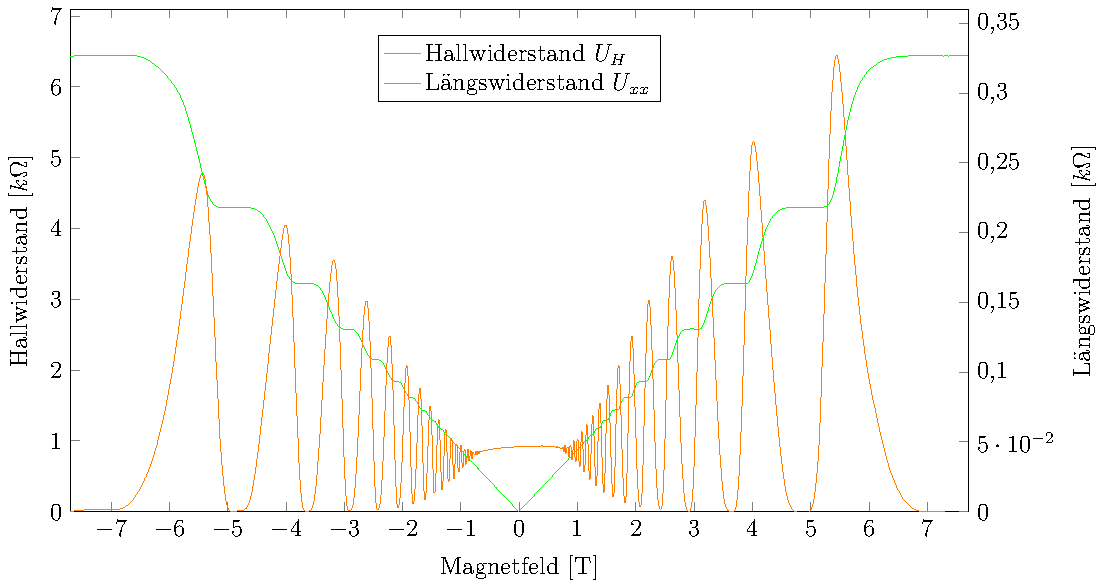
\includegraphics{graphs/ac/full_range.pdf}
	\caption[Wechselstrommessung im maximalen Magnetfeldbereich]{
		Hall-Widerstand und Shubnikov-de Haas Oszillationen eines mit Wechselstrom durchflossenen 2DES.
	}
	\label{fig:full_range_ac}
\end{figure}

\begin{figure}[h]
	\centering
	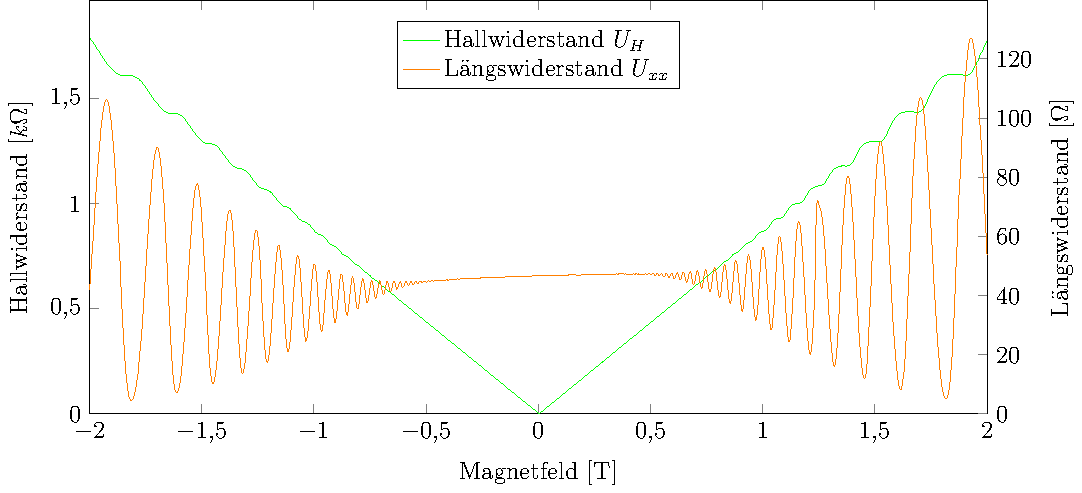
\includegraphics{graphs/ac/pm2T_range.pdf}
	\caption[Höher aufgelöste Wechselstrommessung in Magnetfeldteilbereich]{
		Hall-Widerstand und Shubnikov-de Haas Oszillationen eines mit Wechselstrom durchflossenen 2DES.
	}
	\label{fig:2T_range_ac}
\end{figure}